\documentclass[a4paper]{article}
\title{\textbf{Differentiation of Functions}\\(C001)}
\author{Paul Valentine}
\date{17 March 2020}
\usepackage{amsmath}
\usepackage{amssymb}
\usepackage[margin=2cm]{geometry}
\usepackage{physics}
\usepackage{graphicx}
\begin{document}
\maketitle
\begin{abstract}
This paper develops the concept of differentiation of functions as expressing the rate of change of a function at a point. Firstly the rate of change of single variable functions is considered leading to differentiation of multi variable functions and ending in the concept of a direction derivative. In considering directional derivatives the concept of a vector at a point naturally occurs. 
\end{abstract}
\section{Single Variable}
Let $x\in\mathbb{R}$ and $f(x)\in \mathbb{R} \mid f:x \to f(x)$.\\ \\
Consider the linear approximation of the function $f(x)$ at a point displaced from $x$ by $\delta$. Define the tangent to a point on $f(x)$ as being the line that locally best approximates the rate of change of the function not bisecting $f(x)$ evaluated at that point. Define this rate of change to be $f'(x)$
\begin{align}
f(x+\delta)= f(x) + f'(x)\delta \; \therefore \; f'(x) \approx \frac{f(x+\delta)-f(x)}{\delta} \label{eq1}
\end{align}
This approximation gets more and more accurate as $\delta \to 0$. The rate of change of the function $f(x)$ (w.r.t $x$) is therefore.
\begin{equation}
f'(x)=\displaystyle{\lim_{\delta \to 0}} \frac{f(x+\delta)-f(x)}{\delta}
\end{equation}
The process of differentiation can be viewed as a function $g$ acting on the function $f$ such that $g:f \to f'$. When expressed in this form the differentiation becomes an operator with the notation $\dv{}{x}$.
\begin{equation}
\dv{}{x} :f\to f'
\end{equation}
\section{Multi-variable}
A function $f(x,y) \mid x,y \in \mathbb{R} \mid f(x,y):\mathbb{R}^2 \to \mathbb{R}$ can be viewed as a family of functions $f_x(y):\mathbb{R} \to \mathbb{R}$. For example let $f(x,y)=x+xy+y$. Then $f_a(y)=a+ay+y$ and $f'_a(y)=a+1$. The partial derivative is the whole set of such functions $f'_x(y) = x+1$. This is, in effect the derivative of the function holding $x$ constant. This is given the following general notation.
\begin{equation}
\pdv{}{y} f(x,y)
\end{equation}
This is a partial derivative. Given in this form, the partial derivative is a function that acts on a function to produce a function. The above is effectively the rate of change of the function w.r.t to y only. \\ \\
Consider $f(x,y) = \cos(x)+\sin(y)$ as shown in figure \ref{fig1}.
\begin{figure}[h!]
\centering
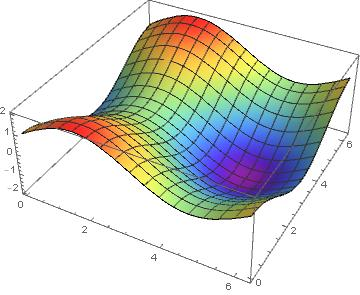
\includegraphics[scale=0.6]{wave.jpg}
\caption{$\cos(x)+ \sin(y)$}
\label{fig1}
\end{figure}
It is clear from this that the function at any point on its surface has distinct rates of change (gradients) in each direction. Therefore to pick out a single rate of change we need to impose a direction on the surface. If we go in any direction we can calculate the change in the function relative to its value at point $p$ from equation \ref{eq1}.
\begin{equation}
\delta f = f_y(x+\delta x)-f_y(x)+f_x(y+\delta y)-f_x(y)= \pdv{f}{x} \delta x + \pdv{f}{y} \delta y \label{eq2}
\end{equation}
In which $\delta x$ and $\delta y$ are components of a displacement vector from point $p$. We parametrise the travel along the vector with a parameter $\lambda \in \mathbb{R}$ such that we can ask what is the rate of change of $f$ w.r.t $\lambda$ as $\lambda \to 0$. This becomes the rate of change at $p$ in the direction of the displacement vector $(\delta z, \delta y)$. Therefore equation \ref{eq2} becomes.
\begin{equation}
\dv{f}{\lambda}=\dv{x}{\lambda} \pdv{f}{x}+ \dv{y}{\lambda} \pdv{f}{y} \label{eq3}
\end{equation}
Equation \ref{eq3} is illuminating if once more we consider differentiation as a function acting on functions.
\begin{equation}
\dv{}{\lambda} f = \dv{x}{\lambda} \pdv{}{x} f+\dv{y}{\lambda} \pdv{}{y} f\label{eq4}
\end{equation}
Equation \ref{eq4} exposes how a vector (in this specific case a displacement vector) $\dv{x}{\lambda} \pdv{}{x} + \dv{y}{\lambda} \pdv{}{y}$ acts on a function $f$ to produce $\dv{f}{\lambda}$. Seen through this lens it is clear that $\dv{}{\lambda}$ is a vector $v$ in the most abstract of senses arising out of consideration of analytical differentiation. A remarkable result! Here, equation \ref{eq4} is a \textbf{Directional Derivative}.
\begin{equation}
\dv{}{\lambda} \bigg\rvert_p : \mathbb{R}^n \to \mathbb{R}
\end{equation}
Thus we can view a vector at a point as forming a linear map of a function to $\mathbb{R}$
\begin{equation}
v_p:f \to \mathbb{R}
\end{equation}
The family of linear maps (vectors) at a point for a tangent space $T_p$ at that point of the same dimension as the function. 
\end{document}